\section{Anforderungen und Konzeption}
\subsection{Anforderungen}
Dieses Kapitel beschreibt die Anforderungen an das Projekt. Das Projekt ist hierbei die Implementierung und die Analyse einer Spiel-KI für das Spiel Ganz schön clever von Anfang bis Ende.
\subsubsection{Rahmenbedingungen}
Der zeitliche Rahmen der Arbeit beträgt vier Monate. In dieser Zeit ist zunächst ein Grundkonzept in Form eines Exposés vorzustellen. Anschließend soll dieses Konzept weiter verfeinert und validiert werden, was schließlich zur Vervollständigung des Projektes mit den gewünschten, sich aber zum Teil auch ändernden Anforderungen führen soll. 

Es ist eine Künstliche Intelligenz zu implementieren, welche das Spiel Ganz schön clever effizient spielen soll. Dazu muss zunächst die Spielumgebung entwickelt und implementiert werden. Mithilfe dieser soll ein Verfahren entwickelt werden, welches die Künstliche Intelligenz in dieser Umgebung trainieren soll.

Anschließend sind die Ergebnisse des Entwicklungsprozesses, sowie des Ereignisses selbst zu analysieren. Dies soll mithilfe geeigneter, schlüssiger und verständlicher Methoden und Visualisierungstechniken erfolgen.
\subsubsection{Das Spiel}
Das Spiel heißt Ganz schön clever. Es ist ein Würfelspiel bei dem es darum geht möglichst viele Punkte innerhalb einer vorgeschriebenen Rundenanzahl zu erreichen [siehe Grundlagen].

Zunächst soll ein Prototyp der Spielumgebung entwickelt werden, welcher später nach und nach erweitert werden soll, bis das Spiel mit all seinen Funktionalitäten implementiert worden ist.\\

Diese Funktionalitäten sind:

Die sechs farbigen Würfel, welche geworfen werden können und zufällig eine Würfelzahl von 1 bis 6 liefern. Es werden dabei immer alle aktuell gültigen Würfel gleichzeitig geworfen.

Einen Mechanismus, welcher die Würfel für die aktuelle Runde als ungültig markiert, sobald sie gewählt werden. Ungültige Würfel dürfen nicht gewählt werden [siehe Grundlagen].

Ein Mechanismus, welcher Würfel mit einer niedrigeren Augenzahl als der aktuell gewählte Würfel als ungültig für die Runde markiert.

Ein Runden-System, bei dem insgesamt sechs Runden gespielt werden, in denen jeweils bis zu drei Würfe erfolgen, falls bei einem der Würfe noch gültige Würfel vorhanden sind. Zudem erfolgt bei nach jeder Runde die Auswahl eines Würfels vom Silbertablett, welches die ungültigen Würfel eines anderen Spielers beinhaltet. Wenn das Spiel alleine gespielt wird und es dadurch keinen anderen Spieler gibt, werden diese Würfel zufällig gewürfelt und dann drei davon per Zufall auf das Silbertablett gelegt. Außerdem werden Boni am Anfang der ersten, zweiten, dritten und vierten Runde für alle Spieler freigeschaltet [siehe Grundlagen].

Die fünf farbigen Felder, gelb, blau, grün, orange und lila. Jedes Feld hat seine eigenen Regeln, wenn es darum geht wann ein Würfel gewählt werden darf, um eines der Subfelder (beziehungsweise Kästchen) auf diesem Feld anzukreuzen [siehe Grundlagen]. Die Felder beinhalten verschiedene Boni, welche freigespielt werden, wenn bestimmte Kästchen oder Kombinationen aus diesen ausgefüllt worden sind [siehe Grundlagen].

Die sieben verschiedenen Boni, Fuchs, Extra Wahl, Neu Würfeln, Gelbes Kreuz, Blaues Kreuz, Grünes Kreuz, Orangene Vier, Orangene Fünf, Orangene Sechs sowie Lila Sechs [siehe Grundlagen]. Damit ist sowohl das Erhalten, Speichern, sowie die Benutzung der Boni gemeint.

Ein Mechanismus, welcher Würfel, welche mithilfe der Extra Wahl Boni gewählt wurden als ungültig markiert, damit diese nicht erneut in der selben Runde durch die Extra Wahl Boni gewählt werden können.

Ein Mechanismus, der Würfel zur richtigen Zeit wieder als gültig markiert. Dies erfolgt nach dem dritten Wurf in der Runde. Nach Extra Wahlen im eigenen Zug (nach dem dritten Wurf). Nach der Wahl vom Silbertablett des Gegners und nach Extra Wahlen, welche nach der Wahl vom Silbertablett des Gegners erfolgen.
\subsubsection{Die Künstliche Intelligenz}
Die Künstliche Intelligenz soll das Spiel möglichst Effizient spielen können. Es sollen geeignete Methoden zur Verfügung stehen, um die KI trainieren und mit ihr nach dem Training Vorhersagen treffen zu können. Außerdem sollte sie Möglichkeiten bieten verschiedene Parameter zu verändern, um den Trainingsprozess zu variieren und zu optimieren. 

Die wichtigsten dieser Parameter sind unter Anderem die Trainingsdauer, welche festlegt wie lange trainiert wird, Gamma, welches bestimmt wie zukunftsorientiert die KI ihre Entscheidungen fällt, die Größe und Art des neuronalen Netzen, das verwendet wird, welches bestimmt wie und präzise Merkmale von der Künstlichen Intelligenz erfasst werden können und einen oder mehrere Faktoren, welche das Ausmaß von Erkundung und Ausbeutung steuern sollen. 

Außerdem soll die Implementierung auf einfache Art und Weise möglich sein, damit der vorhergesehenen zeitliche Rahmen der Arbeit eingehalten werden kann.
\subsection{Konzeption}
In diesem Kapitel wird das Grundkonzept der Künstlichen Intelligenz, sowie der Spielumgebung und deren Zusammenspiel beschrieben.

\begin{minipage}{\linewidth}
	Die Folgende Abbildung zeigt das Zusammenspiel von Spielumgebung und KI während des Trainingsprozesses:
	
	\vspace{0.5cm}
	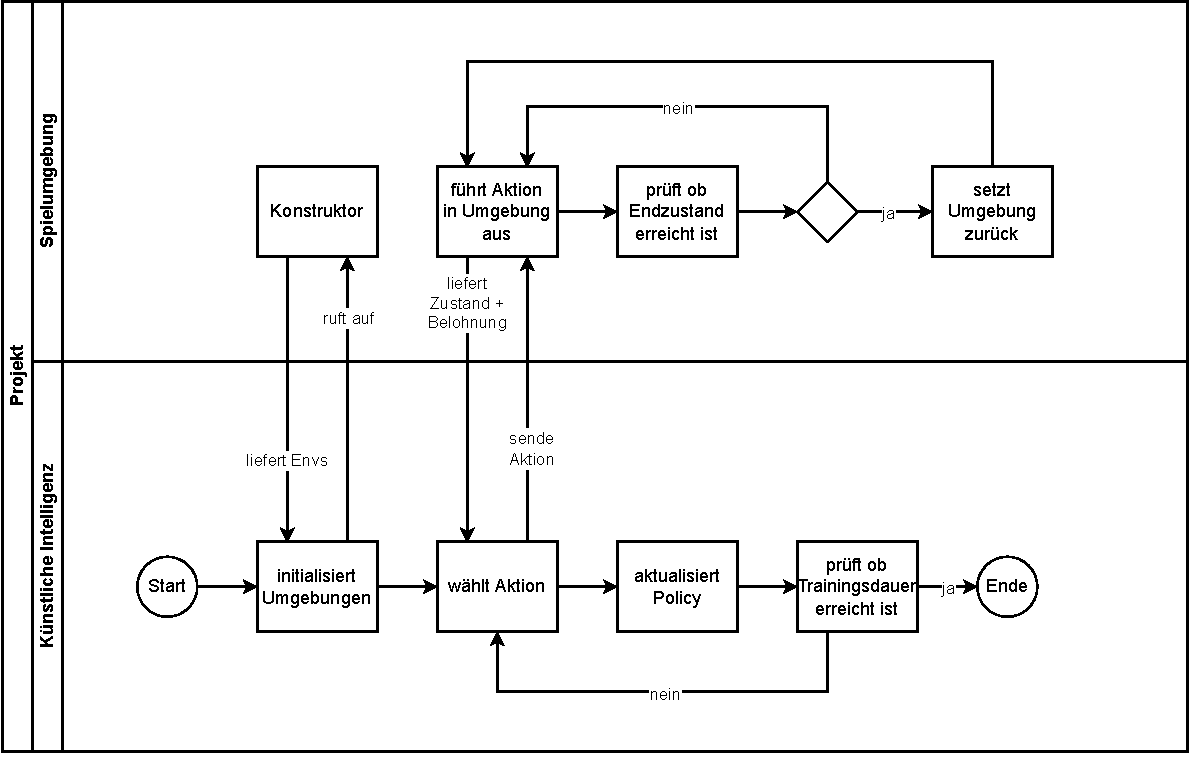
\includegraphics[width=1\textwidth]{Bilder/swimlane.drawio.pdf} 
	
	Abb. 4: Swimlane-Diagramm des Projektes \\

\end{minipage}

Der Trainingsprozess wird angestoßen, die Umgebung beziehungsweise die Umgebungen werden initialisiert. Dazu wird der Konstruktor der Umgebung aufgerufen. Daraufhin wird von der KI eine Aktion ausgewählt und an die Umgebung weitergeleitet. Die Umgebung führt diese Aktion aus und prüft ob der Endzustand des Spiels erreicht worden ist oder nicht. Wenn der Endzustand erreicht wurde wird die Umgebung auf den Anfangszustand zurückgesetzt. Wenn der Endzustand nicht erreicht worden ist, wird der Prozess ohne Weiteres fortgesetzt. Daraufhin liefert die Umgebung der KI eine Belohnung für den ausgeführten Schritt und den neuen Zustand der Umgebung nach Ausführung der Schrittes/der Aktion.

Daraufhin aktualisiert die Künstliche Intelligenz ihr neuronales Netz mit der Policy und überprüft ob bereits genügend Zeit vergangen ist, um das Training zu beenden. Wenn die festgelegte Zeit vergangen ist wird das Training an dieser Stelle beendet. Wenn nicht wird die nächste Aktion gewählt und das Training wird fortgesetzt.

Dies ist lediglich eine vereinfachte Darstellung des Prozesses. In Wirklichkeit wird die Policy nicht nach jedem Schritt/jeder Aktion aktualisiert, sondern es wird erst eine festgelegte Menge an Aktions-Zustands-Paaren gesammelt. Dann wird das neuronale Netz mit dieser Gesamtmenge aktualisiert.
\subsubsection{Die Spielumgebung}
\begin{minipage}{\linewidth}
	Die folgenden beiden Abbildungen zeigen prinzipiellen Funktionsablauf in der Spielumgebung. Dabei wird am Anfang eine Aktion entgegengenommen und am Schluss der neue Zustand dieser Umgebung nach Ausführung der Aktion zurückgegeben:\\
	
	\vspace{0.5cm}
	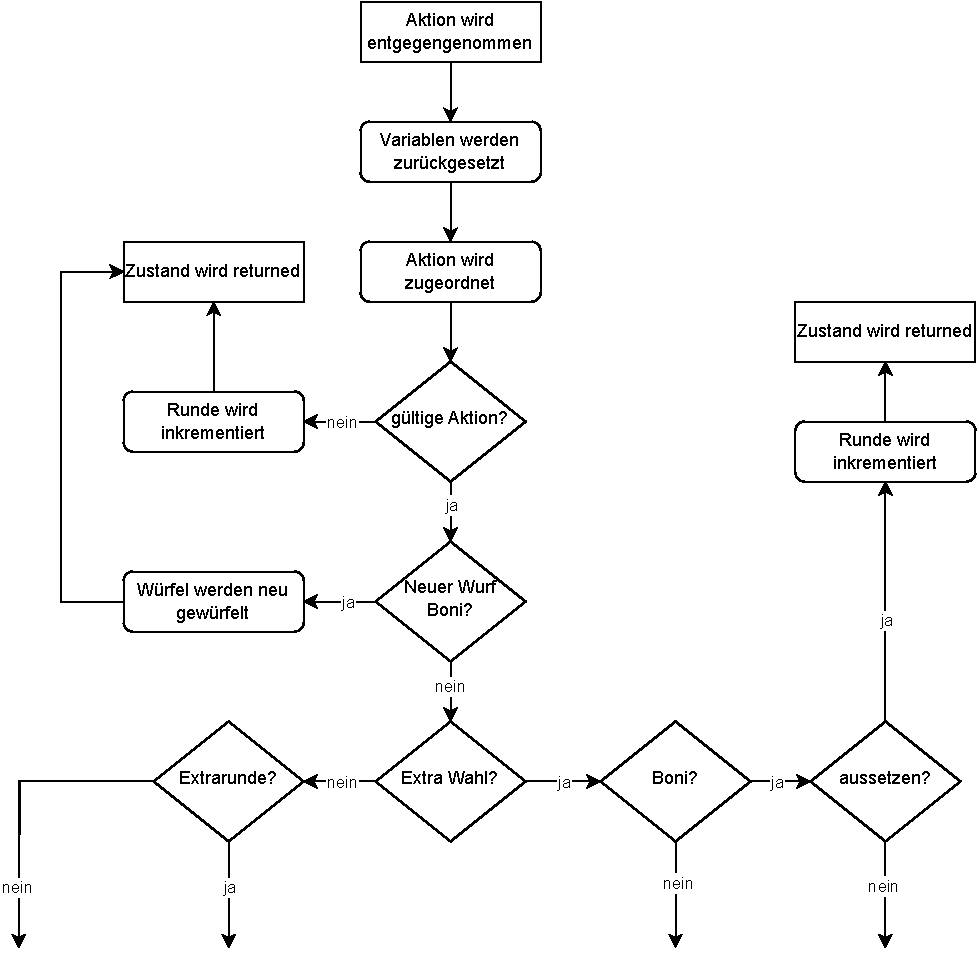
\includegraphics[width=1\textwidth]{Bilder/step3.drawio} 
	
	Abb. 5: Ablauf-Diagramm der Schritt Funktion 1 \\
\end{minipage}

Nachdem die Schritt Funktion angestoßen wird, werden die Variablen dieser Funktion zurückgesetzt, um einen klaren Schnitt zwischen vergangenen Aktionen und der aktuellen Aktion zu erzielen.

Anschließend wird die Aktion ihrem entsprechenden Ablauf zugeordnet. Es gibt Aktionen für Wahlen nach normalen Würfen, für Wahlen von Würfeln des Silbertablettes, sowie für das Nutzen von Boni. Außerdem gibt es eine Aktion, die nur dann wählbar ist, wenn keine der anderen Aktionen gewählt werden kann. Dies ist die Aktion für ungültige Züge.

Ist die Aktion nicht gültig, wird die Runde inkrementiert und der Zustand der Umgebung zurückgegeben.

Wird die Neu Würfeln Boni verwendet, werden die gültigen Würfel neu gewürfelt und anschließend der Zustand zurückgegeben.

Ist beides nicht der Fall kommt es zu einer Auswahl zwischen den wesentlichen Aktionen der Umgebung. Es gibt sogenannte Extra Wahlen, diese spalten sich auf in Extra Wahlen mit der Extra Wahl Boni und Wahlen vom Silbertablett des Mitspielers.

Handelt es sich nicht um eine Extra Wahl, so folgt eine Unterteilung in Extra Runden und Normale Runden. Bei Extra Runden wird eine der Boni verwendet, die es erlauben eines der farbigen Felder auszufüllen [siehe Grundlagen].

Handelt es sich nicht um eine Extrarunde muss es eine normale Wahl nach einem Standardwurf in einer der sechs Runden sein [siehe Grundlagen].

Handelt es sich um eine Extra Wahl mit Boni, dann steht noch die Aktion "aussetzen" zur Wahl. Diese inkrementiert lediglich die Runde, sodass das Spiel weiter fortgesetzt werden kann. Dies spiegelt die Möglichkeit im Spiel wieder auf die Nutzung der Extra Wahl Boni zu verzichten.

Der folgende Ablauf der Funktion gestaltet sich relativ ähnlich bei allen vier Varianten. Bei allen Vieren wird das Feld und das Kästchen ermittel, welches ausgefüllt werden soll und das entsprechende Kästchen wird anschließend ausgefüllt. Dann wird die Belohnung für diesen Schritt ermittelt.

Am Ende der Funktion unterscheiden sich die vier Varianten allerdings wieder. Bei der normalen Wahl nach einem Standardwurf werden die entsprechenden Würfel als ungültig markiert [siehe Grundlagen] und die Runde wird inkrementiert. Außerdem prüft die Funktion bei dieser Variante am Schluss ob das Spiel terminiert ist oder nicht.

Beim ausfüllen eines Feldes mittels Boni (keine Extra Wahl) wird der entsprechende Boni dekrementiert.

Bei der Extra Wahl vom Silbertablett wird die Runde inkrementiert.

Bei der Extra Wahl mittels Boni wird der gewählte Würfel als ungültig markiert und der Extra Wahl Boni wird dekrementiert.

Bei allen vier Varianten wird am Ende der Funktion der aktuelle Zustand der Umgebung sowie die erhaltene Belohnung für den Schritt/die Aktion zurückgegeben.\\

\begin{minipage}{\linewidth}

	\vspace{0.5cm}
	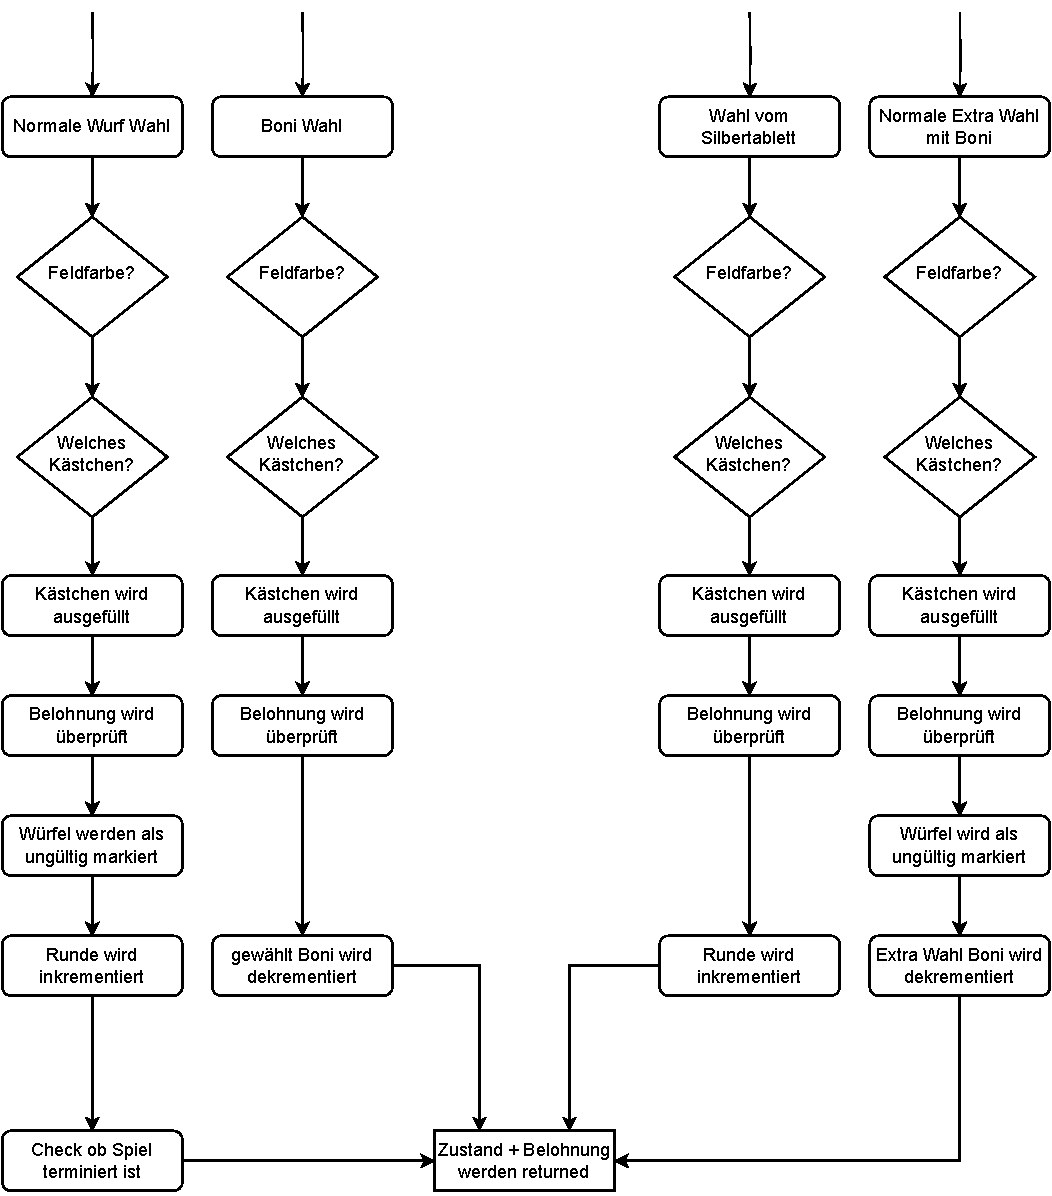
\includegraphics[width=1\textwidth]{Bilder/step2.drawio}
	
	Abb. 6: Ablauf-Diagramm der Schritt Funktion 2 \\
\end{minipage}
\subsubsection{Die Künstliche Intelligenz}
\subsubsection{Einschränkungen}